\documentclass[8pt, xcolor={svgnames}, hyperref={colorlinks,linkcolor=black, citecolor=black, urlcolor=black}]{beamer}


\usepackage[labelfont={color=amethyst,bf}]{caption}
\usetheme[progressbar=frametitle]{metropolis}
\usepackage{appendixnumberbeamer}
\usepackage{url}
\usepackage{booktabs}
\usepackage{braket}
\usepackage[scale=2]{ccicons}
\usepackage{amsfonts} 
\usepackage{amssymb}
\usepackage[english]{babel}
\usepackage{fontawesome}
\usepackage{multicol}
\usepackage{bm}
\usepackage{algorithm}
\usepackage{algpseudocode}
\usepackage{enumitem}

\usepackage[]{pseudo}


\usepackage{tikz}
\usetikzlibrary{positioning,arrows,calc,math,angles,quotes}
\usepackage{blochsphere}

\usetikzlibrary{arrows,automata}
\usetikzlibrary{positioning}
\usetikzlibrary{arrows.meta,
                bending,
                intersections,
                quotes,
                shapes.geometric}

\tikzset{
    state/.style={
           rectangle,
           rounded corners,
           draw=black, very thick,
           minimum height=1em,
           inner sep=2pt,
           text centered,
           },
}


\definecolor{myv}{rgb}{0.36, 0.22, 0.33}
\definecolor{gio}{rgb}{0.45, 0.31, 0.59}
\definecolor{light}{rgb}{0.8, 0.8, 1}
\definecolor{warmblack}{rgb}{0.0, 0.26, 0.26}
\definecolor{brown(web)}{rgb}{0.65, 0.16, 0.16}
\definecolor{cadmiumgreen}{rgb}{0.0, 0.42, 0.24}
\definecolor{darkmidnightblue}{rgb}{0.0, 0.2, 0.4}
\definecolor{brightube}{rgb}{0.82, 0.62, 0.91}

\definecolor{codegreen}{rgb}{0,0.6,0}
\definecolor{codegray}{rgb}{0.5,0.5,0.5}
\definecolor{codepurple}{rgb}{0.58,0,0.82}
\definecolor{backcolour}{rgb}{0.95,0.95,0.92}
\definecolor{amethyst}{rgb}{0.6, 0.4, 0.8}


\definecolor{light-gray}{gray}{0.95}

\newcommand{\code}[1]{\colorbox{light-gray}{\texttt{#1}}}
\newcommand*{\xdash}[1][3em]{\rule[0.5ex]{#1}{0.55pt}}


\usepackage{listings}
\lstdefinestyle{mystyle}{
    backgroundcolor=\color{backcolour},   
    commentstyle=\color{codegreen},
    keywordstyle=\color{codepurple},
    numberstyle=\tiny\color{codepurple},
    stringstyle=\color{magenta},
    basicstyle=\scriptsize,
    breakatwhitespace=false,         
    breaklines=true,                 
    captionpos=b,                    
    keepspaces=true,                 
    numbers=left,                    
    numbersep=5pt,                  
    showspaces=false,                
    showstringspaces=false,
    showtabs=false,                  
    tabsize=2
}

\lstset{style=mystyle}
\usepackage[most]{tcolorbox}
\usepackage{xcolor}

%\usepackage[citecolor = green, linkcolor = blue, bookmarks=true, urlcolor=blue,
%colorlinks=true, pagebackref=true]{hyperref}

%\usepackage{xspace}
\title{Density estimation via Quantum Adiabatic Machine Learning}
\date{Feb. 23, 2023}
\author[Matteo Robbiati]{Matteo Robbiati}



\begin{document}

\begin{frame}{full-stack algorithms with \texttt{qibo}}
\faTerminal\,\, \texttt{qibo} covers all quantum computation areas, thus 
we can implement and test \textbf{full-stack} quantum algorithms.

\begin{figure}
    \includegraphics[width=0.8\textwidth]{figures/full_stack.png}%
    \label{fig:full_stack}
\end{figure}
\end{frame}


\begin{frame}{Full-stack gradient descent}

\faTerminal\,\, \texttt{WORK 1:} hardware-compatible 
    \textbf{quantum gradient descent} (QGD)\footnote{\faBook\,\, 
    \href{https://arxiv.org/abs/2210.10787}{arXiv:2210.10787}}:
\begin{itemize}[noitemsep]
    \item[\tiny\faSquare] implementing parameter-shift rules to evaluate gradients
    on hardware;
    \item[\tiny\faSquare] successfully fitting $y=\sin{2x}$ on TII QPUs.
    \item[\tiny\faSquare] results comparable to a genetic optimization.
\end{itemize}
\begin{figure}
    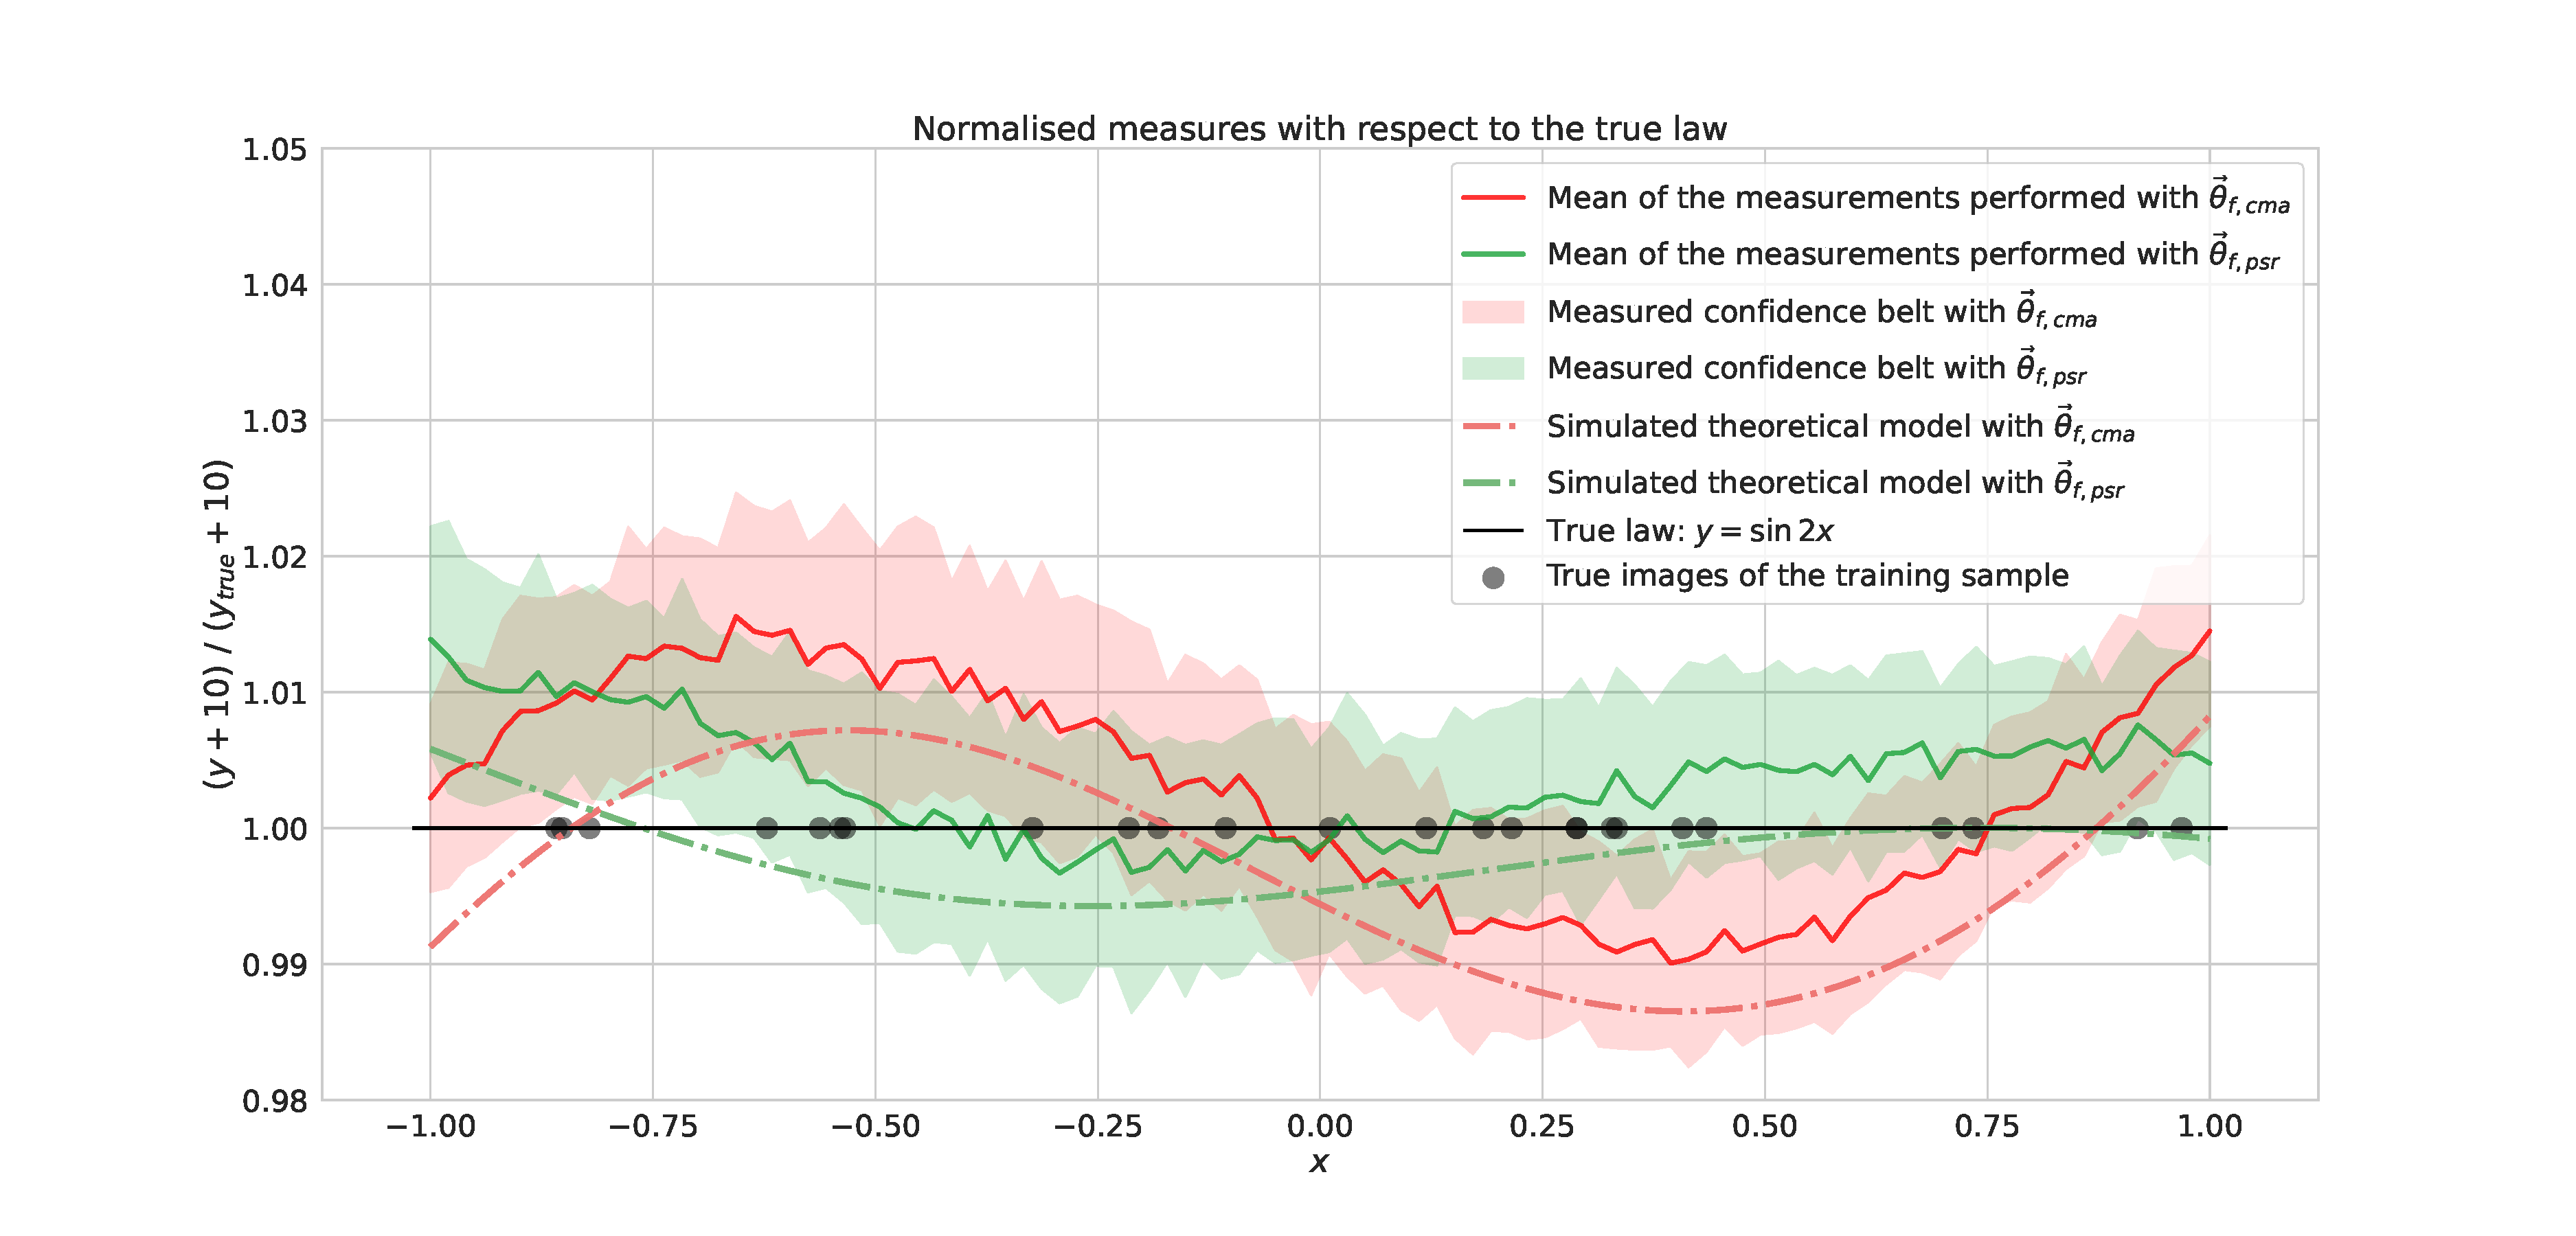
\includegraphics[width=0.8\textwidth]{figures/adam.pdf}%
    \caption{Normalised fit of $y=\sin{2x}$ through a full-stack Adam descent 
    performed using \texttt{qibo}.}
    \label{fig:adam}
\end{figure}

\end{frame}

\begin{frame}{Error mitigation impact on QGD algorithms}


\faTerminal\,\, \texttt{WORK 2:} error mitigation impact during QGD steps:
\begin{itemize}[noitemsep]
    \item[\tiny\faSquare] combine error mitigation with derivation methods we 
    have in \texttt{qibo};
    \item[\tiny\faSquare] successfully fitting High Energy Physics (HEP) quarks parton
    density functions in simulation
    using mitigated-noisy circuits;
    \item[\tiny\faSquare] we are going to run the algorithm on the hardware.
\end{itemize}

\begin{figure}
    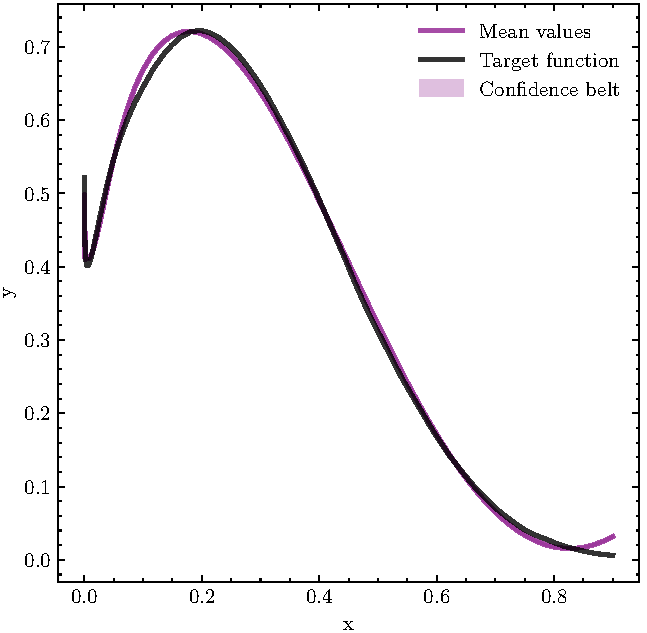
\includegraphics[height=3.5cm, width=0.33\textwidth]{figures/exact.pdf}%
    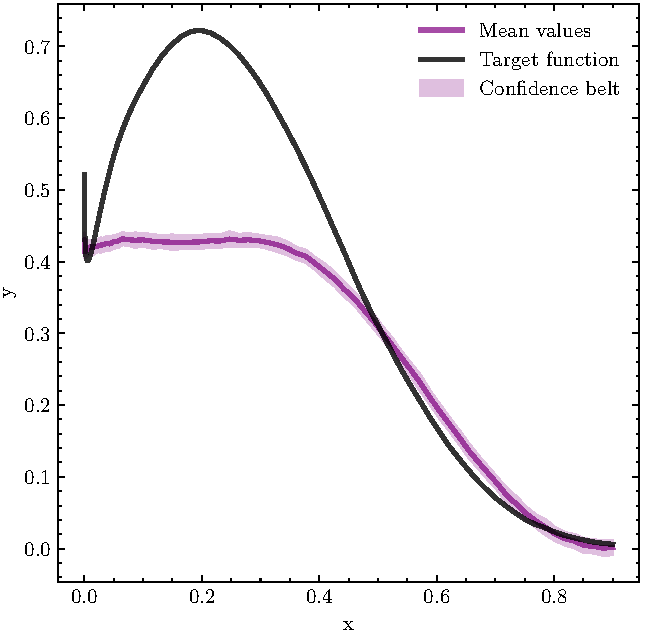
\includegraphics[height=3.5cm, width=0.33\textwidth]{figures/noisy.pdf}%
    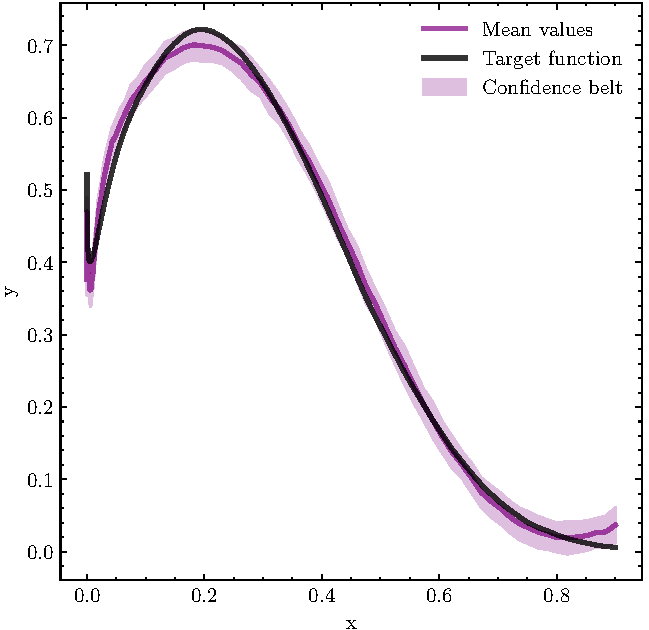
\includegraphics[height=3.5 cm, width=0.33\textwidth]{figures/mitigated.pdf}%
    \caption{PDF fit performed with different levels of noisy simulation. 
    From left to right, exact simulation, noisy simulation, noisy simulation 
    applying error mitigation to the predictions.}
    \label{fig:mitigated_fit}
\end{figure}


\end{frame}

\begin{frame}{Quantum technologies for High Energy Physics (HEP)}
\faTerminal\,\, We cooperate with the 
\href{https://quantum.cern/}{Quantum Techonolgy Initiative} (QTI) at CERN, where 
Matteo is spending the Doctoral program.
\begin{figure}
    
\includegraphics[width=1\textwidth]{figures/qti.png}%
    \label{fig:full_stack}
\end{figure}
\faTerminal\,\, The \texttt{qibo} ecosystem has been presented\footnote{\href{https://indico.cern.ch/event/1235582/}{QTI-TH Forum 2023-01-12}}
and used\footnote{\href{https://indico.cern.ch/event/1235584/}{QTI-TH Forum 2023-01-26}}
during the QTI-TH forum.
\end{frame}


\begin{frame}{Determining PDFs via adiabatic quantum computing}

\faTerminal\,\, \texttt{WORK 3:} we used \texttt{qibo} for testing a new Quantum
Adiabatic Machine Learning (QAML) strategy\footnote{\faBook\,\, \href{https://arxiv.org/abs/2303.11346}{arXiv:2303.11346}}:
\begin{itemize}[noitemsep]
    \item[\tiny\faSquare] we embed a Cumulative Density Function (CDF) into ad adiabatic
    evolution;
    \item[\tiny\faSquare] we translate the adiabatic hamiltonians into circuits;
    \item[\tiny\faSquare] we derivate this circuits with hardware-compatible techniques
    for estimating the Probability Density Function (PDF).
\end{itemize}

\begin{figure}
    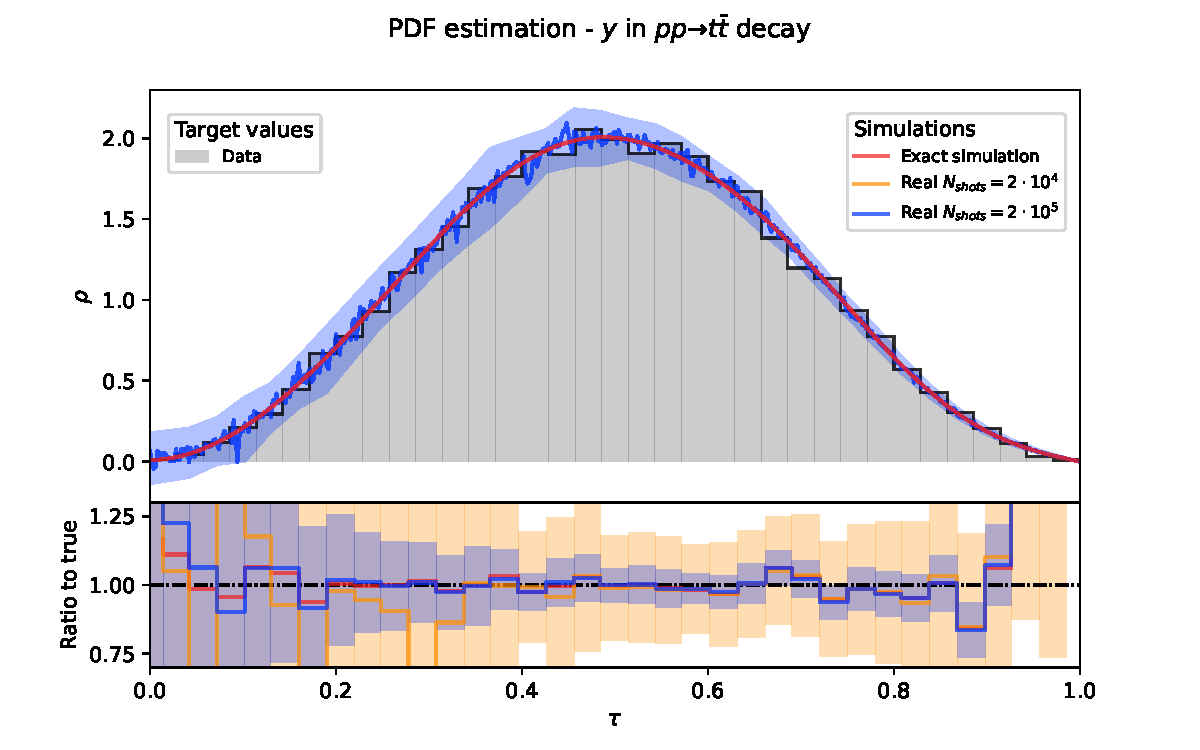
\includegraphics[width=0.5\textwidth]{figures/rapidity.pdf}%
    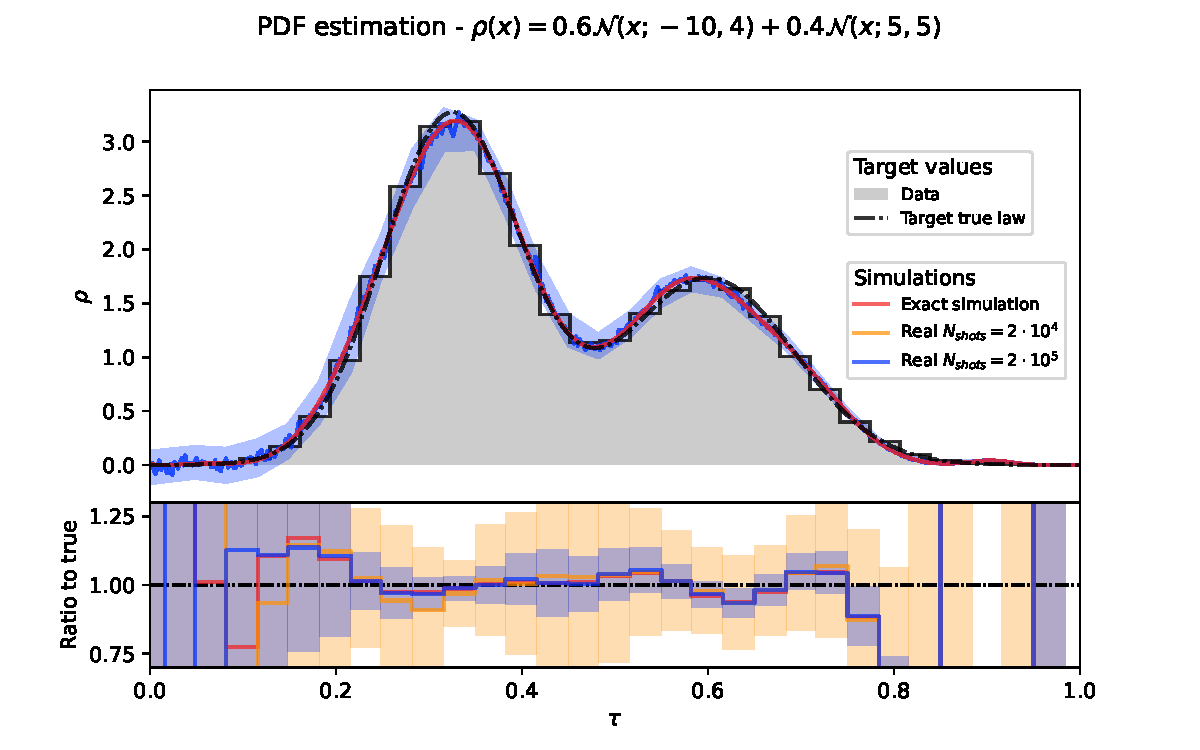
\includegraphics[width=0.5\textwidth]{figures/gauss.pdf}
    \caption{QAML results. On the right PDF fit of rapidity in a $pp\to t\bar{t}$ HEP decay,
    on the left we fit a gaussian mixture.}
    \label{fig:adiabatic_fit}
\end{figure}
\end{frame}

\begin{frame}{Upcoming}

\begin{tcolorbox}[colback=blue!15, title=   \faTerminal\,\, \texttt{WORK 4:} Quantum Analytical integration using the parameter shift rule.]
Given the integral:
\begin{equation}
I = \int_a^b g(x)\, \text{d}x,
\end{equation}
we can use the expectation value of an observable $\hat{B}$ 
to fit $g(x)$;
\begin{equation}
    \hat{g}(x) \equiv \braket{\mathcal{C}(x)} \equiv \braket{\psi_i|\mathcal{C}^{\dagger}(x) |
    \hat{B}\, \mathcal{C}(x)| \psi_i},
\end{equation}
this makes the original circuit $\mathcal{C}$ a good 
estimator of the integral function as $I = \braket{\mathcal{C}(b)}- \braket{\mathcal{C}(a)}$ 
due to the fundamental theorem of integral calculus.
\end{tcolorbox}

\begin{tcolorbox}[colback=red!15, title=\faTerminal\,\, \texttt{WORK 5:} How to classify HEP event topology
using a quantum annealer?]
We had an interesting discussion during the QTI-TH Forum\footnote{\href{https://indico.cern.ch/event/1267029/}{QTI-TH Forum 2023-03-30}}
about the topic and we are thinking to use \texttt{qibo} for approaching this task. 
\end{tcolorbox}
\end{frame}

\end{document}